\underline{Gaz doskonały} - zwany też gazem idealnym, jest to abstrakcyjny, matematyczny model fizyczny gazu, spełniający następujące warunki: 

\begin{enumerate}[-]
	\item brak oddziaływań miedzycząsteczkowych z wyjątkiem odpychania w momencie zderzeń cząsteczek,
	\item objętość cząsteczek jest znikoma w stosunku do objętości gazu.
	\item zderzenia cząsteczek są doskonale sprężyste,
	\item cząsteczki znajdują się w ciągłym, chaotycznym ruchu.
\end{enumerate}

\underline{Rozkład Maxwella} – wzór określający rozkład prędkości cząstek gazu doskonałego. Założenie:  funkcja rozkładu f zależy tylko od wartości prędkości v:\newline
$ f(v_x,v_y,v_z) = f(v_x^2+v_y^2+v_z^2) $\newline
Żaden kierunek nie jest uprzywilejowany, ruch w każdym z kierunków x,y i z odbywa się niezależnie:\newline
$ f(v_x,v_y,v_z) = h(v_x)h(v_y)h(v_z) $\newline
Funkcja rozkładu h jest taka sama dla każdego kierunku co wynika z symetrii.\newline
$ ln[h(v_x)] + ln[h(v_y)] + ln[h(v_z)] = ln[f(v_x^2+v_y^2+v_z^2)] $, stąd:\newline
$ h(v_x) = C_xe^{(-Bv_x^2)} $\newline
$ f(v) = C_xC_yC_ze^{-B(v_x^2+v_y^2+v_z^2)} = Ce^{-Bv^2} $\newline
Stałą C znajdziemy z warunku normalizacji natomiast stałą B znajdujemy na podstawie równania łączącego średni kwadrat prędkości cząsteczek z temperaturą oraz wyrazić wartość średnią kwadratu prędkości poprzez funkcję gęstości prawdopodobieństwa:\newline
$ \frac{m<v^2>}{2} = \frac{3}{2}kT = \frac{m}{2}\int_{0}^{\infty} v^2f(v)*4\pi v^2dv $, gdzie:
$ m $ - masa cząsteczki,\newline
$ k $ - stała Boltzmanna,\newline
$ 4\pi v^2dv $ - element objętości przestrzeni prędkości (v, v+dv) we współrzędnych sferycznych.\newline
Otrzymujemy ostatecznie:\newline
$ f(v) = (\frac{m}{2\pi kT})^{\frac{3}{2}}e^{\frac{mv^2}{2kT}} $\newline
$ \frac{dP}{dv} = 4\pi (\frac{m}{2\pi kT})^{\frac{3}{2}}v^2e^{\frac{mv^2}{2kT}} $ - gęstość prawdopodobieństwa wystąpienia cząsteczki o prędkości v.\newline
Rozkład Maxwella pokazuje, że prędkości cząsteczek zależą od temperatury oraz masy molowej. Wraz ze wzrostem temperatury rozkład się poszerza (rysunek~\ref{maxwellDistribution}), a jego prędkość najbardziej prawdopodobna (tam gdzie dP/dv jest największe), jak i średnia prędkość (<v>) oraz średnia prędkość kwadratowa ($ \sqrt{<v^2>} $) zwiększają się.

\begin{figure} [H]
	\centering
	\begin{subfigure}{1.0\textwidth}
		\centering
		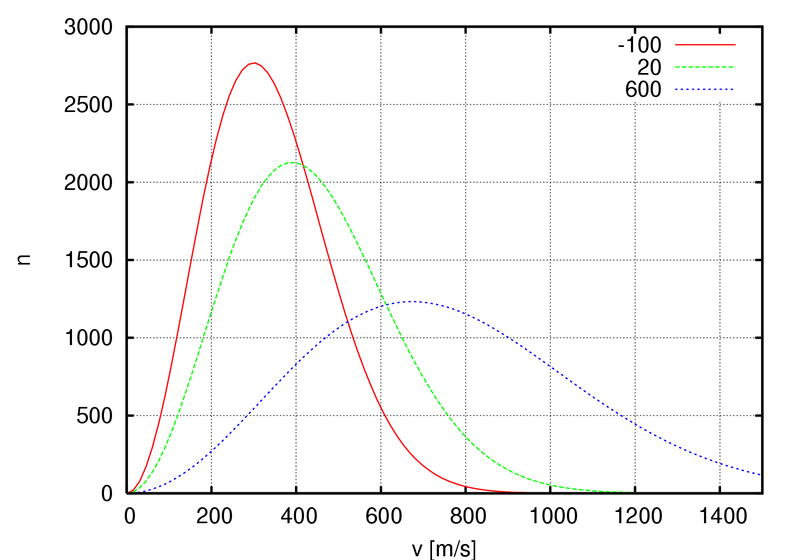
\includegraphics[width=0.98\linewidth]{generalIssues/Figures/maxwellDistribution.png}
	\end{subfigure}
	\caption{Rozkład Maxwella dla tlenu dla trzech temperatur (–100 $ ^\circ C $, temperatura pokojowa i 600 $ ^\circ C $). Wartość funkcji odpowiada liczbie cząsteczek spośród 1 miliona cząsteczek, jaka będzie poruszać się z prędkością v+/-0,5 m/s.}
	\label{maxwellDistribution}
\end{figure}

Wzór na koncentrację cząsteczek, czyli ich liczbę w jednostce objętości:\newline
$ n = n_0\exp(-\frac{E_p}{kT}) $, gdzie:\newline
$ E_p $ - energia potencjalna cząstek w danym stanie (np. na danej wysokości),\newline
$ n_0 $ - koncentracja cząsteczek dla $ E_p = 0 $ (np. koncentracja na powierzchni ziemi).\newline

Wzór ten wyraża zależność koncentracji cząsteczek od ich wysokości lub energii potencjalnej. Wynikający z niego rozkład koncentracji nosi nazwę rozkładu Boltzmanna i odnosi się nie tylko do pola sił przyciągania ziemskiego, ale do dowolnego pola potencjalnego, jeśli tylko cząsteczki poruszają się chaotycznym ruchem cieplnym. Liczba cząsteczek w objętości $ dV = dz \cdot dy \cdot dz $, której położenie określają współrzędne $ (x,y,z) $ wynosi:\newline
$ dn(x,y,z) = n_0\exp(-\frac{E_p(x,y,z)}{kT})dx\cdot dy\cdot dz $\newline
Nietrudno tu zauważyć podobieństwo rozkładów Maxwella i Boltzmanna, z tą różnicą, że pierwszy wyraża zależność od kwadratu prędkości lub energii kinetycznej, drugi - od energii potencjalnej. Rozkład zawierający obie te zależności nosi nazwę rozkładu Maxwella-Boltzmanna i ma postać:
$ dn(x,y,z,v_x,v_y,v_z) = A\exp(-\frac{E_p+E_k}{kt})dx\cdot dy \cdot dz \cdot v_x \cdot v_y \cdot v_z $

\underline{Zakaz Pauliego} głosi, że prawdopodobieństwo znalezienia w układzie fermionów (cząstek o spinie połówkowym) pary cząstek o jednakowych liczbach kwantowych jest równe zeru (czyli np. możemy znaleść na tej samej orbicie atomowej dwa elektrony, ale muszą mieć przeciwne spiny - jest to przykład degeneracji).

Zgodnie z rozkładem Fermiego-Diraca (rysunek~\ref{fermi})średnia liczba cząstek w niezdegenerowanym stanie energetycznym $ E $ dana jest przez:\newline

$ <n> = \dfrac{1}{e^{\beta (E-\mu)}+1} $, gdzie:\newline
$ E $ - energia tego stanu,\newline
$ \mu $ - potencjał chemiczny,\newline
$ \beta = 1/k_bT $\newline

\begin{figure} [H]
	\centering
	\begin{subfigure}{1.0\textwidth}
		\centering
		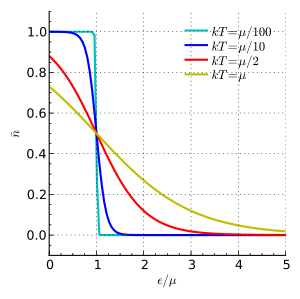
\includegraphics[width=0.7\linewidth]{generalIssues/Figures/fermi.png}
	\end{subfigure}
	\caption{Rozkład Fermiego-Diraca. Oś pozioma: $ E/\mu $. Oś pionowa: $ <n> $.}
	\label{fermi}
\end{figure}

W temperaturze zera bezwzględnego wprowadza się oznaczenie $ \mu = \mu(0) = E_F $ - jest to energia najwyżej obsadzonego stanu ($ k_F $ - poziom Fermiego) w temperaturze zera bezwzględnego. W tej temperaturze obsadzone są wszystkie stany o energii mniejszej lub równej energii Fermiego ($ E_F $ a wyższe stany nie są obsadzone.Dla każdej temperatury $ T $ zachodzi $ P(E_k) = 0.5 $ gdy $ E_k = \mu $. Dla takich energii, że $ E_k - \mu \gg k_BT $ rozkład przechodzi w klasyczny rozkład Boltzmanna.

Statystyka Bosego-Einsteina dotyczy bozonów (cząstek o spinie całkowitym, których nie obowiązuje zakaz Pauliego) traktowanych jako gaz bozonowy. Zgodnie z rozkładem Bosego-Einsteina średnia liczba cząstek w danym stanie kwantowym jest równa:

$ <n_i> = \dfrac{n}{Z}\dfrac{g_i}{e^{\beta(E_i-\mu)}-1} $, gdzie:\newline
$ E_i $ - energia i-tego stanu,\newline
$ g_i $ - degeneracja i-tego stanu,\newline
$ n $ - całkowita liczba cząstek,\newline
$ \mu $ - potencjał chemiczny,\newline
$ Z = \sum_{i}\dfrac{g_i}{e^{\beta(E_i-\mu)}-1} $ - suma statystyczna.\newline
Potencjał chemiczny w tym rozkładzie jest zawsze ujemny lub równy zeru. Gdy temperatura jest wysoka, można zaniedbać składnik –1 i rozkład przechodzi w rozkład fizyki klasycznej - klasyczny rozkład Boltzmanna. Rozkładowi Bosego-Einsteina podlegają fotony (o spinie 1) – nosi on wtedy nazwę rozkładu Plancka, który tłumaczy promieniowanie ciała doskonale czarnego. Jego wprowadzenie przez Plancka zapoczątkowało mechanikę kwantową. Zakaz Pauliego nie dotyczy bozonów, umożliwia to ich kondensację.
\underline{Kondensacja Bosego-Einsteina} – efekt kwantowy zachodzący w układach podległych rozkładowi Bosego-Einsteina. W temperaturach niższych od temperatury krytycznej część cząstek (bozonów) przechodzi w zerowy stan pędowy – cząstki te mają identyczny pęd. Oznacza to, że w zerowej objętości przestrzeni pędów może znajdować się niezerowa liczba cząstek. Mówi się wtedy o makroskopowym obsadzeniu stanu podstawowego. Efektem kondensacji jest kolektywne zachowanie wszystkich cząstek biorących w niej udział (w przybliżeniu wszystkie zachowują się jak jedna cząstka). Nie chodzi tu o kondensację w zwykłym sensie w przestrzeni położeniowej – cząstki nie znajdują się w jednym miejscu, lecz o "kondensację" cząstek w przestrzeni pędów – znaczna liczba cząstek ma taki sam pęd. Rozkład przestrzenny cząstek "skondensowanych" pozostaje równomierny (jeśli nie ma pól zewnętrznych). W kondensacie Bosego-Einsteina zachodzi zjawisko nadciekłości. 
